

\tikzset{every picture/.style={line width=0.75pt}} %set default line width to 0.75pt        

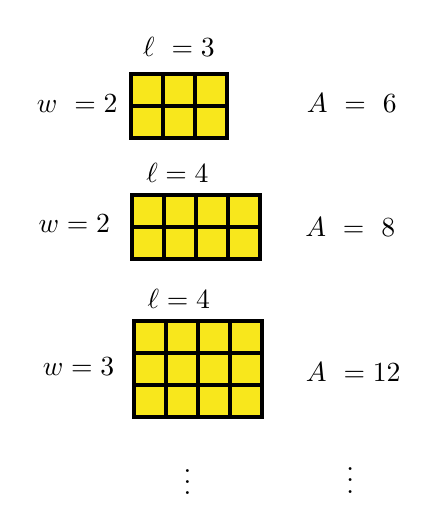
\begin{tikzpicture}[x=0.75pt,y=0.75pt,yscale=-1,xscale=1,scale=0.7]
%uncomment if require: \path (0,338); %set diagram left start at 0, and has height of 338

%Shape: Square [id:dp38271822688596946] 
\draw  [fill={rgb, 255:red, 248; green, 231; blue, 28 }  ,fill opacity=1 ][line width=1.5]  (189,34) -- (211,34) -- (211,56) -- (189,56) -- cycle ;
%Shape: Square [id:dp8679439248883813] 
\draw  [fill={rgb, 255:red, 248; green, 231; blue, 28 }  ,fill opacity=1 ][line width=1.5]  (211,34) -- (233,34) -- (233,56) -- (211,56) -- cycle ;
%Shape: Square [id:dp3558050933364425] 
\draw  [fill={rgb, 255:red, 248; green, 231; blue, 28 }  ,fill opacity=1 ][line width=1.5]  (233,34) -- (255,34) -- (255,56) -- (233,56) -- cycle ;
%Shape: Square [id:dp8748116538918442] 
\draw  [fill={rgb, 255:red, 248; green, 231; blue, 28 }  ,fill opacity=1 ][line width=1.5]  (189,56) -- (211,56) -- (211,78) -- (189,78) -- cycle ;
%Shape: Square [id:dp06759803167989387] 
\draw  [fill={rgb, 255:red, 248; green, 231; blue, 28 }  ,fill opacity=1 ][line width=1.5]  (211,56) -- (233,56) -- (233,78) -- (211,78) -- cycle ;
%Shape: Square [id:dp3172857824306643] 
\draw  [fill={rgb, 255:red, 248; green, 231; blue, 28 }  ,fill opacity=1 ][line width=1.5]  (233,56) -- (255,56) -- (255,78) -- (233,78) -- cycle ;
%Shape: Square [id:dp9771058827150725] 
\draw  [fill={rgb, 255:red, 248; green, 231; blue, 28 }  ,fill opacity=1 ][line width=1.5]  (190,117) -- (212,117) -- (212,139) -- (190,139) -- cycle ;
%Shape: Square [id:dp10490248151810566] 
\draw  [fill={rgb, 255:red, 248; green, 231; blue, 28 }  ,fill opacity=1 ][line width=1.5]  (212,117) -- (234,117) -- (234,139) -- (212,139) -- cycle ;
%Shape: Square [id:dp8310609107018645] 
\draw  [fill={rgb, 255:red, 248; green, 231; blue, 28 }  ,fill opacity=1 ][line width=1.5]  (234,117) -- (256,117) -- (256,139) -- (234,139) -- cycle ;
%Shape: Square [id:dp5473468611089647] 
\draw  [fill={rgb, 255:red, 248; green, 231; blue, 28 }  ,fill opacity=1 ][line width=1.5]  (190,139) -- (212,139) -- (212,161) -- (190,161) -- cycle ;
%Shape: Square [id:dp12474790550517523] 
\draw  [fill={rgb, 255:red, 248; green, 231; blue, 28 }  ,fill opacity=1 ][line width=1.5]  (212,139) -- (234,139) -- (234,161) -- (212,161) -- cycle ;
%Shape: Square [id:dp34696767252717375] 
\draw  [fill={rgb, 255:red, 248; green, 231; blue, 28 }  ,fill opacity=1 ][line width=1.5]  (234,139) -- (256,139) -- (256,161) -- (234,161) -- cycle ;
%Shape: Square [id:dp13867107777486232] 
\draw  [fill={rgb, 255:red, 248; green, 231; blue, 28 }  ,fill opacity=1 ][line width=1.5]  (256,117) -- (278,117) -- (278,139) -- (256,139) -- cycle ;
%Shape: Square [id:dp5849236655713153] 
\draw  [fill={rgb, 255:red, 248; green, 231; blue, 28 }  ,fill opacity=1 ][line width=1.5]  (256,139) -- (278,139) -- (278,161) -- (256,161) -- cycle ;
%Shape: Square [id:dp7422021146428393] 
\draw  [fill={rgb, 255:red, 248; green, 231; blue, 28 }  ,fill opacity=1 ][line width=1.5]  (191,204) -- (213,204) -- (213,226) -- (191,226) -- cycle ;
%Shape: Square [id:dp8646869287162122] 
\draw  [fill={rgb, 255:red, 248; green, 231; blue, 28 }  ,fill opacity=1 ][line width=1.5]  (213,204) -- (235,204) -- (235,226) -- (213,226) -- cycle ;
%Shape: Square [id:dp436268216442143] 
\draw  [fill={rgb, 255:red, 248; green, 231; blue, 28 }  ,fill opacity=1 ][line width=1.5]  (235,204) -- (257,204) -- (257,226) -- (235,226) -- cycle ;
%Shape: Square [id:dp40039453862710905] 
\draw  [fill={rgb, 255:red, 248; green, 231; blue, 28 }  ,fill opacity=1 ][line width=1.5]  (191,226) -- (213,226) -- (213,248) -- (191,248) -- cycle ;
%Shape: Square [id:dp34900812081397414] 
\draw  [fill={rgb, 255:red, 248; green, 231; blue, 28 }  ,fill opacity=1 ][line width=1.5]  (213,226) -- (235,226) -- (235,248) -- (213,248) -- cycle ;
%Shape: Square [id:dp6134216351528443] 
\draw  [fill={rgb, 255:red, 248; green, 231; blue, 28 }  ,fill opacity=1 ][line width=1.5]  (235,226) -- (257,226) -- (257,248) -- (235,248) -- cycle ;
%Shape: Square [id:dp2972790637499185] 
\draw  [fill={rgb, 255:red, 248; green, 231; blue, 28 }  ,fill opacity=1 ][line width=1.5]  (257,204) -- (279,204) -- (279,226) -- (257,226) -- cycle ;
%Shape: Square [id:dp6141269163406937] 
\draw  [fill={rgb, 255:red, 248; green, 231; blue, 28 }  ,fill opacity=1 ][line width=1.5]  (257,226) -- (279,226) -- (279,248) -- (257,248) -- cycle ;
%Shape: Square [id:dp04871647434354265] 
\draw  [fill={rgb, 255:red, 248; green, 231; blue, 28 }  ,fill opacity=1 ][line width=1.5]  (191,248) -- (213,248) -- (213,270) -- (191,270) -- cycle ;
%Shape: Square [id:dp6693543844606036] 
\draw  [fill={rgb, 255:red, 248; green, 231; blue, 28 }  ,fill opacity=1 ][line width=1.5]  (213,248) -- (235,248) -- (235,270) -- (213,270) -- cycle ;
%Shape: Square [id:dp25950883575769756] 
\draw  [fill={rgb, 255:red, 248; green, 231; blue, 28 }  ,fill opacity=1 ][line width=1.5]  (235,248) -- (257,248) -- (257,270) -- (235,270) -- cycle ;
%Shape: Square [id:dp5668503605566757] 
\draw  [fill={rgb, 255:red, 248; green, 231; blue, 28 }  ,fill opacity=1 ][line width=1.5]  (257,248) -- (279,248) -- (279,270) -- (257,270) -- cycle ;

% Text Node
\draw (222,15) node   {$\ell \ =3$};
% Text Node
\draw (152,54) node   {$w\ =2$};
% Text Node
\draw (341,54) node   {$A\ =\ 6$};
% Text Node
\draw (221,102) node   {$\ell =4$};
% Text Node
\draw (150,137) node   {$w=2$};
% Text Node
\draw (340,139) node   {$A\ =\ 8$};
% Text Node
\draw (222,189) node   {$\ell =4$};
% Text Node
\draw (153,235) node   {$w=3$};
% Text Node
\draw (342,239) node   {$A\ =12$};
% Text Node
\draw (228,309) node   {$\boldsymbol{\vdots }$};
% Text Node
\draw (340,308) node   {$\boldsymbol{\vdots }$};


\end{tikzpicture}